\chapter{Advanced Data Representation}
\label{chap:advanced_data_representation}

\begin{figure}[ht]
	\hfill
	\begin{minipage}{0.5\textwidth}
		\centering
		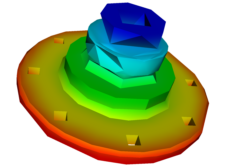
\includegraphics{VTKTextbook-158}\\
		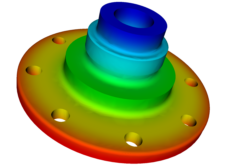
\includegraphics{VTKTextbook-157}
		\caption*{\texttt{Adaptive tessellation of higher-order cells.}}
	\end{minipage}
\end{figure}


\firstletter{T}his chapter examines advanced topics in data representation.
Topics include topological and geometric relationships and computational methods for cells and datasets.

\section{Coordinate Systems}
We will examine three different coordinate systems: the global, dataset, and structured coordinate systems.
Figure8–1 shows the relationship between the global and dataset coordinate systems, and depicts the structured coordinate system.

\subsection{Global Coordinate System}
The global coordinate system is a Cartesian, three-dimensional space. Each point is expressed as a triplet of values $(x,y,z)$ along the $x$, $y$, and $z$ axes.
This is the same system that was described in Chapter 3 (see \ref{sec:coordinate_systems}).
The global coordinate system is always used to specify dataset geometry (i.e., the point coordinates),and data attributes such as normals and vectors.
We will use the word ``position'' to indicate that we are using global coordinates.

\section{Searching}
\label{sec:searching}
Searching is an operation to find the cell containing a specified point \emph{p}, or to locate cells or points in a region surrounding \emph{p}.
Algorithms requiring this operation include streamline generation, where we need to find the starting location within a cell; probing, where the data values at a point are interpolated from the containing cell; or collision detection, where cells in a certain region must be evaluated for intersection.
Sometimes (e.g., image datasets), searching is a simple operation because of the regularity of data. However, in less structured data, the searching operation is more complex.

To find the cell containing \emph{p}, we can use the following naive search procedure.
Traverse all cells in the dataset, finding the one (if any) that contains \emph{p}.
To determine whether a cell contains a point, the cell interpolation functions are evaluated for the parametric coordinates $(r,s,t)$.
If these coordinates lie within the cell, then \emph{p} lies in the cell.
The basic assumption here is that cells do not overlap, so that at most a single cell contains the given point \emph{p}.
To determine cells or points lying in the region surrounding \emph{p}, we can traverse cells or points to see whether they lie within the region around \emph{p}.
For example, we can choose to define the region as a sphere centered at \emph{p}.
Then, if a point or the points composing a cell lie in the sphere, the point or cell is considered to be in the region surrounding \emph{p}.

\section{Putting It All Together}
In this section we will finish our earlier description of an implementation for unstructured data. We also define a high-level, abstract interface for cells and datasets. This interface allows us to implement the general (i.e., dataset specific) algorithms in the \emph{Visualization Toolkit}. We also describe
implementations for color scalars, searching and picking, and conclude with a series of examples to demonstrate some of these concepts.

\subsection{Picking}
\label{subsec:picking}

The Visualization Toolkit provides a variety of classes to perform actor (or vtkProp), point, cell, and
world point picking ( Figure8–38 ).

\subsection{Point Probe}
\label{subsec:point_probe}